
\documentclass{beamer}

\usepackage{beamerthemesplit}
\usepackage{graphics}
\usepackage{graphicx}
\usepackage{hyperref}

% pie charting
\usepackage{calc}
\usepackage{ifthen}
\usepackage{tikz}
\usepackage{textpos}

\definecolor{links}{HTML}{2A1B81}
\hypersetup{urlcolor=links} % Does not apply color to href's
\hypersetup{colorlinks,linkcolor=,linkbordercolor=,urlcolor=links,urlbordercolor=links,pdfborderstyle={/S/U/W 1}}

\setbeamertemplate{navigation symbols}{}%remove navigation symbols

\title[RaBe Technik-Gruppe]{RaBe Mitgliederversammlung 2013}
\author{Lucas S. Bickel\\{ hairmare@purplehaze.ch}}
\institute[]{Radio Bern, Technik-Gruppe}
\date[DLT 2012]{L\"anggass-Tr\"aff, 2013-04-03}
\subject{RaBe Vollversammlung 2013, IT}

\begin{document}

  \frame
  {

    \titlepage

    \begin{textblock*}{200pt}(0pt,-120pt)
      \scalebox{0.175}
      {
        
\includegraphics[trim = 200pt 0pt 155pt 0pt,clip]{img/logo.png}
      }
    \end{textblock*}
  }

  \section*{Aus der Technik}
  \frame{
    \center{Aus der Technik}
  }

  \subsection*{Probleme}

  \frame
  {
    \frametitle{Probleme}
    
    \begin{itemize}
    \item{USB Buchsen im Studio}
    \item{Knackserprobleme Infokabine}
    \item{2 HDs im Server ersetzt}
    \item{Stromversorgung}
    \end{itemize}
  }

  \subsection*{\"Anderungen}

  \frame
  {
    \center{\"Anderungen}
  }

  \frame
  {
    \frametitle{\"Anderungen}

    \begin{itemize}
    \item{USV und Stromsituation}
    \item{neue Player PCs in den Studios}
    \item{Ausbau Netzwerk am Randweg}
    \item{Umbau Songticker, neu mit Sendungslinks}
    \item{Fernzugriff f\"ur Programmkommision via WebDAV}
    \end{itemize}
  }

  \subsection*{Live-\"Ubertragungen}

  \frame
  {
    \center{Live-\"Ubertragungen}
  }

  \frame
  {
    \frametitle{Live-\"Ubertragungen}

    \begin{itemize}
    \item{Tour de Lorraine}
    \item{Openair am Bielersee, erste \"Ubertragung via Satellit}
    \item{RaBe Fest 2013}
    \end{itemize}
  }

  \subsection*{Aktuelles}

  \frame
  {
    \center{Aktuelles}
  }

  \frame
  {
    \frametitle{Aktuelles}
    
    \begin{itemize}
    \item{Stellennetz IT-Praktikum}
    \item{WLAN am Randweg}
    \end{itemize}
  }

  \section*{Einblick in den Technik-Alltag}

  \subsection*{MP3 Streaming}

  \frame
  {
    \center{MP3 Streaming}
  }

  \frame
  {
    \frametitle{Anzahl H\"orer Anfangs 2012}

    \begin{figure}
    \resizebox{300pt}{150pt}
    {
      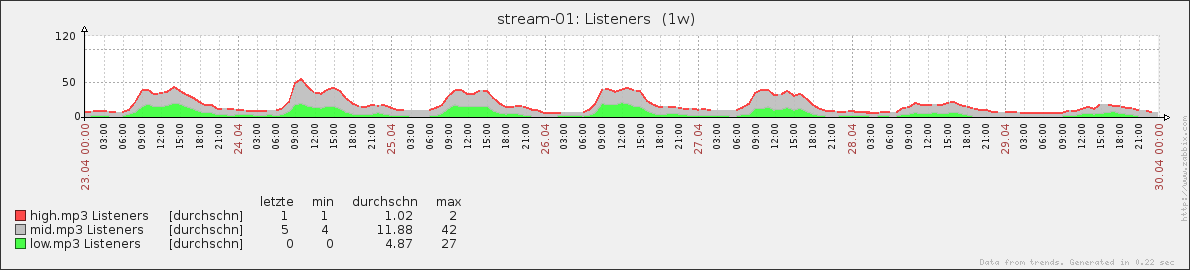
\includegraphics[trim = 86pt 152pt 30pt 35pt, clip]{img/stream-2012.png}
    }
    \end{figure}
  }

  \frame
  {
    \frametitle{Anzahl H\"orer vorletzte Woche}
    
    \begin{figure}
    \resizebox{300pt}{150pt}
    {
      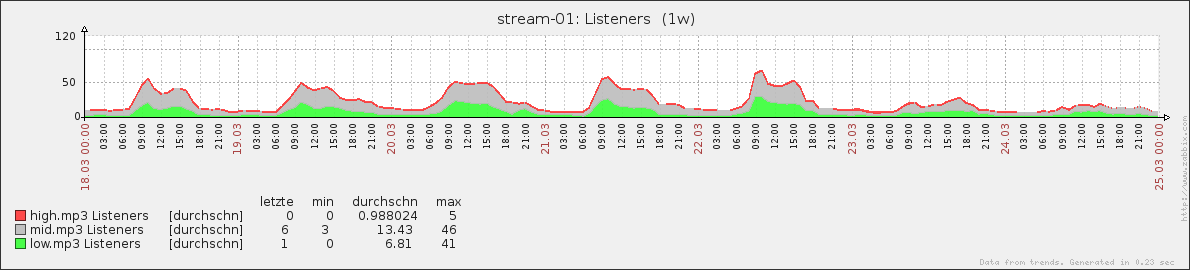
\includegraphics[trim = 86pt 152pt 30pt 35pt, clip]{img/stream-2013.png}
    }
    \end{figure}
  }

  \subsection*{Speicherplatz}

  \frame
  {
    \center{Speicherplatz}
  }

  \frame
  {
    \frametitle{Aufteilung Speicherplatz}

    \begin{itemize}
    \item{ca. 13.5 TiB Platz, davon ca. 8 TiB frei}
    \end{itemize}

    \scalebox{0.32}
    {
      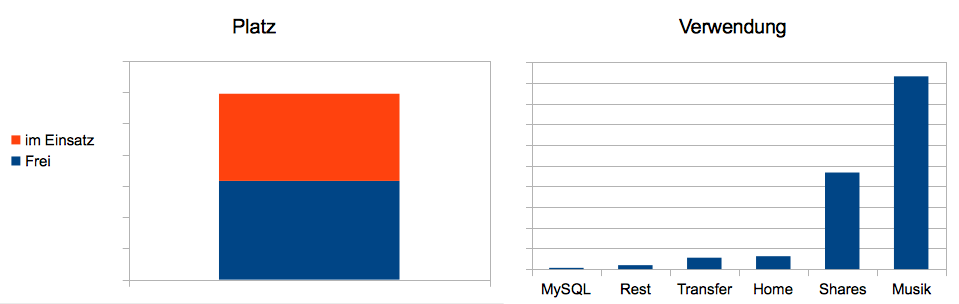
\includegraphics{img/hd-verwendung.png}
    }
  }

  \frame
  {
    \center{HD-Management im Server-Umfeld}
  }

  \frame
  {
    \frametitle{HD-Management im Server-Umfeld}
    
    \begin{itemize}
    \item{7 HDs werden gekauft}
    \end{itemize}

    \resizebox{40pt}{40pt}
    {
      
\includegraphics{img/hdd_big_unknown.png}
    }
    \resizebox{40pt}{40pt}
    {
      
\includegraphics{img/hdd_big_unknown.png}
    }
    \resizebox{40pt}{40pt}
    {
      
\includegraphics{img/hdd_big_unknown.png}
    }
    \resizebox{40pt}{40pt}
    {
      
\includegraphics{img/hdd_big_unknown.png}
    }
    \resizebox{40pt}{40pt}
    {
      
\includegraphics{img/hdd_big_unknown.png}
    }
    \resizebox{40pt}{40pt}
    {
      
\includegraphics{img/hdd_big_unknown.png}
    }
    \resizebox{40pt}{40pt}
    {
      
\includegraphics{img/hdd_big_unknown.png}
    }
  }

  \frame
  {
    \frametitle{HD-Management im Server-Umfeld}

    \begin{itemize}
    \item{6 davon eingebaut}
    \end{itemize}

    \resizebox{40pt}{40pt}
    {
      
\includegraphics{img/hdd_big_ok.png}
    }
    \resizebox{40pt}{40pt}
    {
      
\includegraphics{img/hdd_big_ok.png}
    }
    \resizebox{40pt}{40pt}
    {
      
\includegraphics{img/hdd_big_ok.png}
    }
    \resizebox{40pt}{40pt}
    {
      
\includegraphics{img/hdd_big_ok.png}
    }
    \resizebox{40pt}{40pt}
    {
      
\includegraphics{img/hdd_big_ok.png}
    }
    \resizebox{40pt}{40pt}
    {
      
\includegraphics{img/hdd_big_ok.png}
    }
    \resizebox{40pt}{40pt}
    {
      
\includegraphics{img/hdd_big_unknown.png}
    }
  }

  \frame
  {
    \frametitle{HD-Management im Server-Umfeld}

    \begin{itemize}
    \item{Eine steigt aus}
    \end{itemize}

    \resizebox{40pt}{40pt}
    {
      
\includegraphics{img/hdd_big_critical.png}
    }
    \resizebox{40pt}{40pt}
    {
      
\includegraphics{img/hdd_big_ok.png}
    }
    \resizebox{40pt}{40pt}
    {
      
\includegraphics{img/hdd_big_ok.png}
    }
    \resizebox{40pt}{40pt}
    {
      
\includegraphics{img/hdd_big_ok.png}
    }
    \resizebox{40pt}{40pt}
    {
      
\includegraphics{img/hdd_big_ok.png}
    }
    \resizebox{40pt}{40pt}
    {
      
\includegraphics{img/hdd_big_ok.png}
    }
    \resizebox{40pt}{40pt}
    {
      
\includegraphics{img/hdd_big_unknown.png}
    }
  }

  \frame
  {
    \frametitle{HD-Management im Server-Umfeld}

    \begin{itemize}
    \item{und wird zeitnahe ersetzt}
    \end{itemize}

    \resizebox{40pt}{40pt}
    {
      
\includegraphics{img/hdd_big_critical.png}
    }
    \resizebox{40pt}{40pt}
    {
      
\includegraphics{img/hdd_big_ok.png}
    }
    \resizebox{40pt}{40pt}
    {
      
\includegraphics{img/hdd_big_ok.png}
    }
    \resizebox{40pt}{40pt}
    {
      
\includegraphics{img/hdd_big_ok.png}
    }
    \resizebox{40pt}{40pt}
    {
      
\includegraphics{img/hdd_big_ok.png}
    }
    \resizebox{40pt}{40pt}
    {
      
\includegraphics{img/hdd_big_ok.png}
    }
    \resizebox{40pt}{40pt}
    {
      
\includegraphics{img/hdd_big_ok.png}
    }
  }

  \frame
  {
    \frametitle{HD-Management im Server-Umfeld}

    \begin{itemize}
    \item{die Kaputte geht an den Hersteller}
    \end{itemize}

    \resizebox{40pt}{40pt}
    {
      
\includegraphics{img/hdd_big_error.png}
    }
    \resizebox{40pt}{40pt}
    {
      
\includegraphics{img/hdd_big_ok.png}
    }
    \resizebox{40pt}{40pt}
    {
      
\includegraphics{img/hdd_big_ok.png}
    }
    \resizebox{40pt}{40pt}
    {
      
\includegraphics{img/hdd_big_ok.png}
    }
    \resizebox{40pt}{40pt}
    {
      
\includegraphics{img/hdd_big_ok.png}
    }
    \resizebox{40pt}{40pt}
    {
      
\includegraphics{img/hdd_big_ok.png}
    }
    \resizebox{40pt}{40pt}
    {
      
\includegraphics{img/hdd_big_ok.png}
    }
  }

  \frame
  {
    \frametitle{HD-Management im Server-Umfeld}

    \begin{itemize}
    \item{sie hat Garantie und wird  ersetzt}
    \end{itemize}

    \resizebox{40pt}{40pt}
    {
      
\includegraphics{img/hdd_big_unknown.png}
    }
    \resizebox{40pt}{40pt}
    {
      
\includegraphics{img/hdd_big_ok.png}
    }
    \resizebox{40pt}{40pt}
    {
      
\includegraphics{img/hdd_big_ok.png}
    }
    \resizebox{40pt}{40pt}
    {
      
\includegraphics{img/hdd_big_ok.png}
    }
    \resizebox{40pt}{40pt}
    {
      
\includegraphics{img/hdd_big_ok.png}
    }
    \resizebox{40pt}{40pt}
    {
      
\includegraphics{img/hdd_big_ok.png}
    }
    \resizebox{40pt}{40pt}
    {
      
\includegraphics{img/hdd_big_ok.png}
    }
  }

  \section*{}
  \subsection*{}

  \frame
  {
    \frametitle{Fragen? Mehr Infos?}

    \begin{itemize}
    \item{Protokolle, usw. im Intranet: \hyperref{https://intranet.rabe.ch}{}{}{intranet.rabe.ch}}
    \item{Neu auch im Web: \hyperref{http://tech.rabe.ch}{}{}{tech.rabe.ch}}
    \item{oder klassisch, per Email: \hyperref{mailto:it@rabe.ch}{}{}{it@rabe.ch}}
    \item{Quelltext dieser Pr\"asentation: \hyperref{https://github.com/radiorabe}{}{}{github.com/radiorabe}}
    \end{itemize}
    
  }
  \frame{
    \center
    {
      \scalebox{0.175}
      {
        
\includegraphics[trim = 200pt 0pt 155pt 0pt,clip]{img/logo.png}
      }
    }
  }

\end{document}

